\documentclass[12pt, a4paper, oneside]{ctexart}
\usepackage{amsmath, amsthm, amssymb, bm, graphicx, hyperref, mathrsfs}

\title{\textbf{科研课堂课程作业}}
\author{黄伟宁}
\date{\today}
\linespread{1.5}
\newcounter{problemname}
\newenvironment{problem}{\stepcounter{problemname}\par\noindent\textbf{题目\arabic{problemname}. }}{\\\par}
\newenvironment{solution}{\par\noindent\textbf{解答. }}{\\\par}
\newenvironment{note}{\par\noindent\textbf{题目\arabic{problemname}的注记. }}{\\\par}
\usepackage{geometry}
\geometry{left=2.54cm,right=2.54cm,top=3.18cm,bottom=3.18cm}

\begin{document}

\maketitle

\begin{problem}
写出KdV方程双孤子解(24)和(25)的推导过程并画图
\end{problem}

\begin{solution}
    方程(14)等价于$ -2F_{2,xt}-2F_{2,xxxx}=B(F_{1} \cdot F_{1} )  $,代入$ F_{1} =e^{\theta_{1} } +e^{\theta_{2} } ,\theta_{i} =k_{i} x-k_{i} ^{3} t-\eta_{i}  $ 有
    \begin{align*}
          & B(F_{1} \cdot F_{1} )                                                                         \\
        = & (D_{x} D_{t} +D_{x}^{4}  )(F_{1} \cdot F_{1} )                                                \\
        = & 2F_{1,xt} F_{1} -2F_{1,x} F_{1,t} +2F_{1,xxxx}F_{1}  -8F_{1,xxx} F_{1,x} +6F_{1,xx} F_{1,xx}  \\
        = & (-6k_{1} k_{2} ^{3} +12k_{1} ^{2} k_{2} ^{2} -6k_{1} ^{3} k_{2}  )e^{\theta_{1} +\theta_{2} }
    \end{align*}
    代入$ F_{2} =a_{12} e^{\theta_{1} +\theta_{2} } $ 有
    \begin{align*}
          & -2F_{2,xt} -2F_{2,xxxx}                                                                             \\
        = & -2a_{12} (3k_{1} ^{3} k_{2} +6k_{1} ^{2} k_{2} ^{2} +3k_{1} k_{2} ^{3} )e^{\theta_{1} +\theta_{2} }
    \end{align*}
    比较等式两端系数即可得到
    $$
        a_{12} =\frac{(k_{1} -k_{2} )^{2} }{(k_{1} +k_{2} )^{2} }
    $$
    以下给出$ k_{1} =1,\eta_{1} =0,k_{2} =2,\eta_{2} =0 $ 时双孤子解的图形(图1):
    \begin{figure}
        \centering
        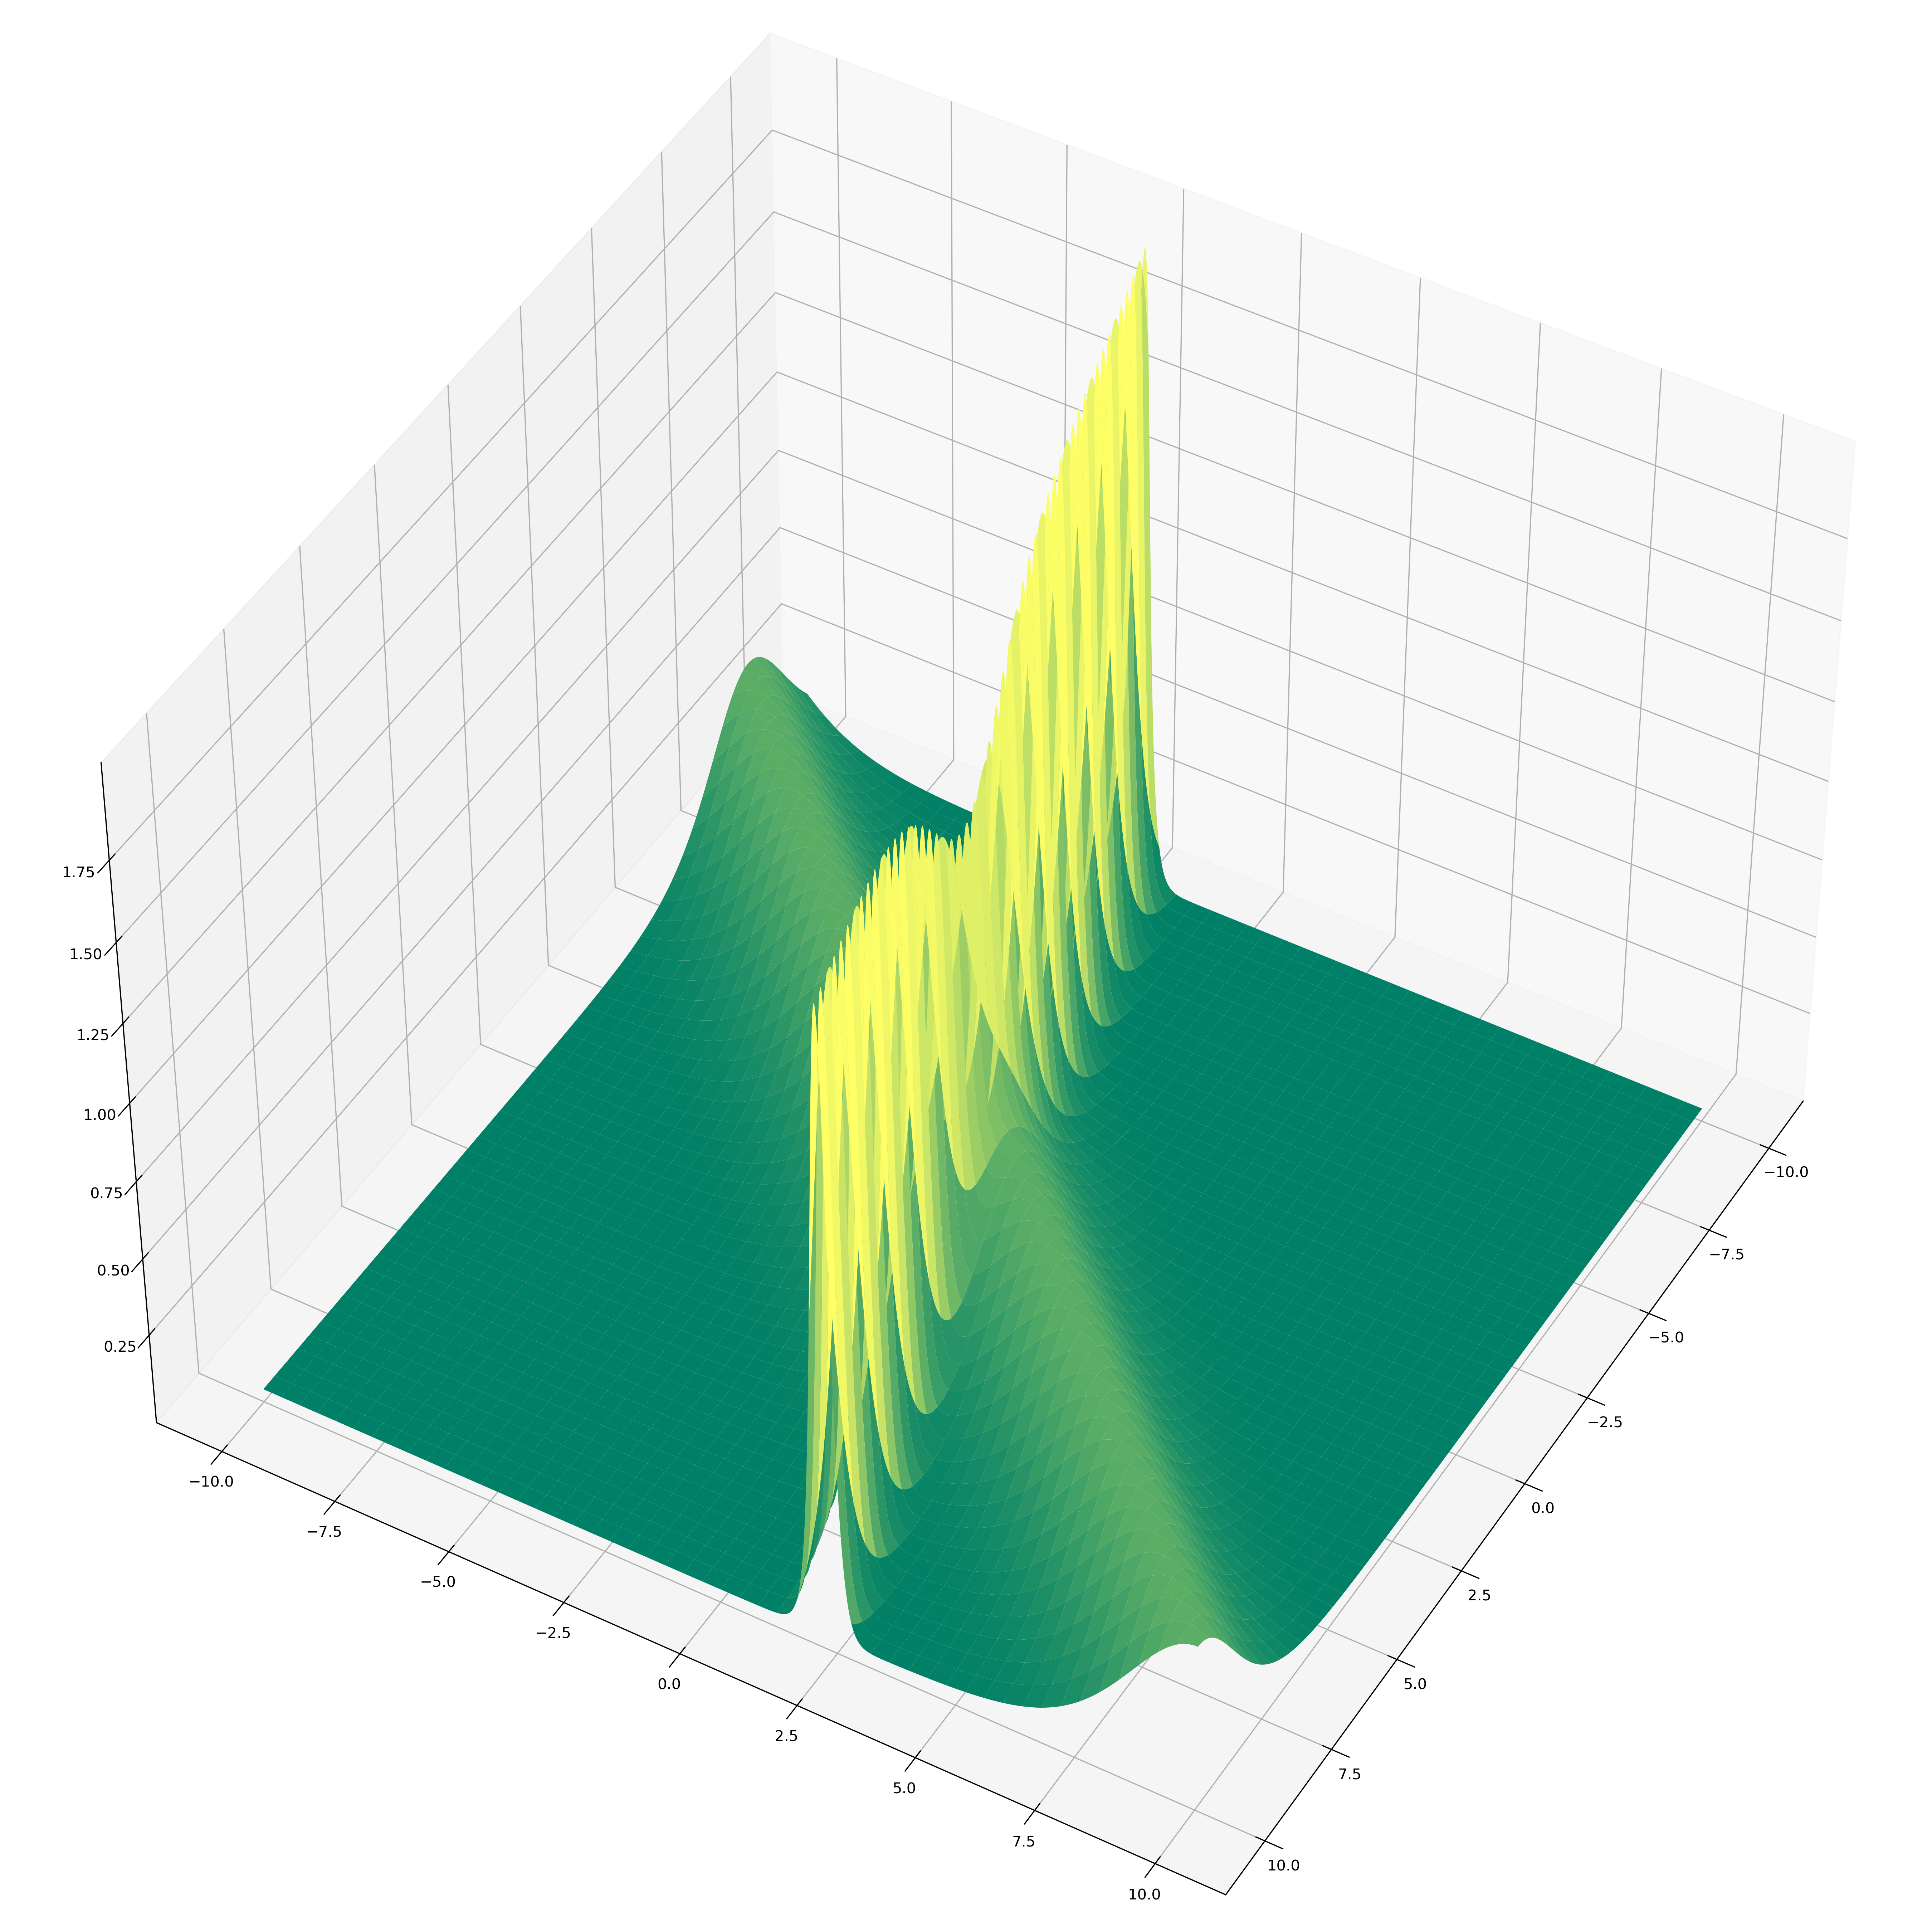
\includegraphics[scale=0.2]{picture/双孤子解.png}
        \caption{双孤子解}
    \end{figure}
\end{solution}

\begin{problem}
用符号计算验证方程(6)的六次多项式解(34),并用tex写出推导过程
\end{problem}

\begin{solution}
    略
\end{solution}
\end{document}